\chapter{Zadanie 1}
\thispagestyle{chapterBeginStyle}
\label{rozdzial1}

\section{Opis problemu}
Zadanie polega na zaimplementowaniu algorytmu 2-aproksymacyjnego, opartym na programowaniu liniowym w języku \textbf{julia} z użyciem pakietu
\textbf{JuMP}, dla problemu szeregowania zadań na niezależnych maszynach z kryterium minimalizacji długości uszeregowania
(ang.  Scheduling on Unrelated Parallel Machines and Makespan Criterion). Danymi są 
zadania $J$, maszyny $M$, oraz czas wykonywania $p_{j,i}$ zadania $j$ na maszynie $i$, celem jest 
zminimalizowanie czasu wykonania wszystkich zadań.
Dane:
\begin{itemize}
    \item $J = \{1,2,3,...,n\}$ - zbiór zadań,
    \item $M = \{1,2,3,...,m\}$ - zbiór maszyn,
    \item $p_{j,i}$ gdzie $j \in J$, $i \in M$ - koszt wykonania zadania $j$ na maszynie $i$.
\end{itemize}

\section{Opis algorytmu}
By rozwiązać problem posłużono się algorytmem podanym w książce \textit{Approximation Algorithms-Springer-Verlag Berlin Heidelberg (2003)}.
Składa się on z podprogramów:

\begin{itemize}
    \item wyliczenia wstępnego - słyży do wyliczenia przedziału w którym będzie stosować przeszukiwanie binarne.
    \item przeszukiwania binarnego na przedziale $[\alpha / m, \alpha]$,
    \item programowania liniowego z podanymi parametrami z przeszukiwania binarnego,
    \item operacji na grafie w celu stworzenia rozwiązania dopuszczalnego.
\end{itemize}
Wyliczenie wstępne obliczające $$\alpha = \sum_{j \in J} min( p_{j,i} : i \in M) $$
to znaczy suma minimalnego kosztu zadań na jakiejś maszynie. 

Przeszukiwanie binarne na przedziale $[\alpha / m, \alpha]$, iteratorem jest wartość $T$,
polega na uruchomieniu programu LP z parametrem $T$ i znalezieniu najmniejszej możliwej wartości
$T$ z którym program LP znalazł rozwiązanie. 

Programowanie liniowe z parametrami:
\begin{itemize}
    \item $T$ - maksymalny koszt pojedynczego zadania, maksymalny koszt na jednej maszynie,
    \item $J$ - zbior zadań,
    \item $M$ - zbiór maszyn,
    \item $p_{j,i}$ - koszt zadania $j$ na maszynie $i$.
\end{itemize}

Model rozwiązujący posiada:
\begin{itemize}
    \item Zmienną $X_{j,i} \geq 0$ - mówiącą w jakim stopniu zadanie $j$ jest przydzielone do maszyny $i$,
    \item Funkcje celu $min \rightarrow \sum_{j \in J, i \in M} X_{j,i} * p_{j,i}$,
    \item Ograniczenie $\forall \substack{j \in J \\ i \in M \\ p_{j,i} > T} X_{j,i} = 0 $ - ogranicza maszynozadania które mają za duży czas wykonania,
    \item Ogarniczenie $\forall \substack{j \in J} \sum_{i \in M} X_{j,i} = 1$ - każde zadania musi zostać wykonane w całości,
    \item Ogarniczenie $\forall \substack{i \in M} \sum_{j \in J} X_{j,i} * p_{j,i} \leq T$ - ogranicza koszt całkowity na jednej maszynie.
\end{itemize}

Program wykorzystuje relaksacje zmiennych, by nie był problemem całkowitoliczbowym. Dzięki temu staje się
algorytmem wielomianowym, ale samo rozwiązania zadania LP, nie musi dawać rozwiązania poprawnego.
Powodem tego jest to że pojedyncze zadanie może być przydzielone częściowo do różnych maszyn, co w rzeczywistości 
nie daje rozwiązania dopuszczalnego. 

Po znalezieniu najmniejszej wartości $T$ oraz rozwiązania LP, trzeba naprawić rozwiązanie.
\begin{itemize}
    \item zadania przydzielone w całości do konkretnej maszyny, przechodzą do rozwiązania,
    \item zadania częściowo przydzielone do różnych maszyn przechodzą do algorytmu grafowego.
\end{itemize}

Algorytm grafowy, rozwiązuje konflikty pomiędzy pojedynczymi zadaniami rozłożonymi na różnych maszynach.
Zadania częściowe posiadają conajmniej dwie maszyny, algorytm rozwiązania konfilktu polega na 
przypisaniu maszynie z jednym zadaniem częściowym, tego zadania i usuniciu zadania z puli częściowych.
Jeżeli powstanie cykl $m-j-m-j$ wybieramy na przemian maszyne do której zostanie przydzielony, 
powtarzamy całość aż wszystkie zadania częściowe staną się przydzielone. 

\section{Wyniki i interpretacja}

Do przetestowania rozwiązania posłużono się danymi z \textit{http://soa.iti.es/problem-instances} do podanego problemu.
Dane zostały podzielone siedem grup, po dwieście przykładów w których jest podział na ilosć
zadań, maszyn i numer zestawu (np. 1025 - 10 oznacza setki zadań tzn. 10 * 100 zadań, 25 - oznacza 20 maszyn 5 - 
 zestaw danych; 554 - 500 zadań, 50 maszyn, 4 zestaw danych; 520 - oznacza 500 zadań, 10 maszyn, 10 zestaw danych):
\begin{itemize}
    \item \textit{instancias1a100} - czas wykonywania zadania jest z przedziału $[1,2,...,100]$,
    \item \textit{instancias100a120} - czas wykonywania zadania jest z przedziału $[100,101,...,120]$,
    \item \textit{instancias100a200} - czas wykonywania zadania jest z przedziału $[100,101,...,200]$,
    \item \textit{instancias10a100} - czas wykonywania zadania jest z przedziału $[10,11,...,100]$,
    \item \textit{instancias1000a1100} - czas wykonywania zadania jest z przedziału $[1000,1001,...,1100]$,
    \item \textit{JobsCorre} - czas wykonywania jest wszczególności zmienny względem zadania,
    \item \textit{MaqCorre} - czas wykonywania jest wszczególności zmienny względem maszyny,
\end{itemize}
Wyniki zostały porównane z wynikami na stronie \textit{http://soa.iti.es/problem-instances}.
Wykresy z danych \textit{instancias} są bardzo zbliżone do siebie. Jak widać algorytm lepiej działa w przypadku
gdy wiele zadań przydzielone jest do jednej maszyny. Dane testowe textit{JobsCorre} wnioski podobne.
Dla danych testowych textit{MaqCorre} algorytm działa bardzo zbliżenie do tego podanego w rozwiązaniu. 
Wyniki wszystkich testów załączony jest w załączniku. 


\begin{figure}[h]
    \centering
    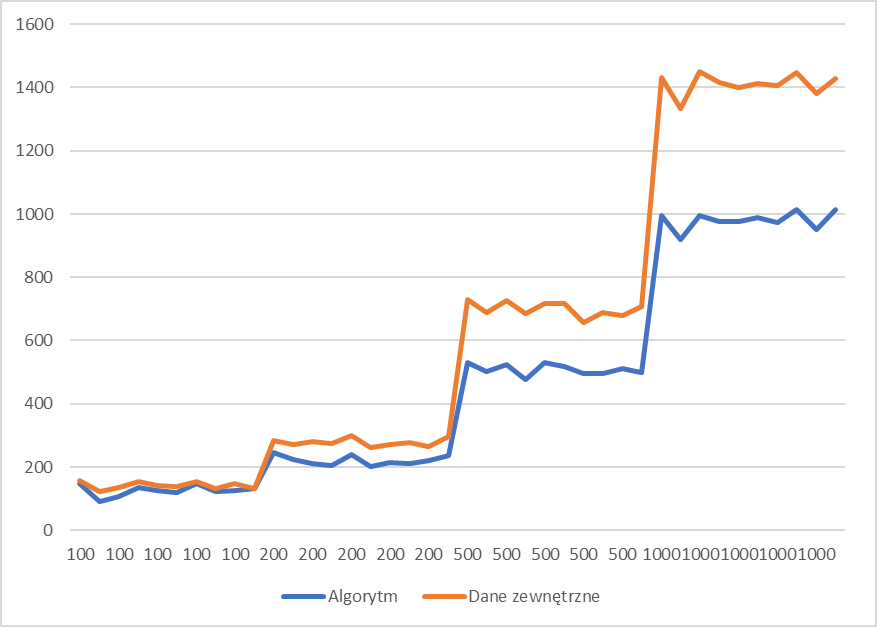
\includegraphics[scale=0.3]{1-100_10.png}
    \caption{Dane dla 1 - 100 z 10 maszynami}
    \label{1-100_10}
\end{figure}



\begin{figure}[h]
    \centering
    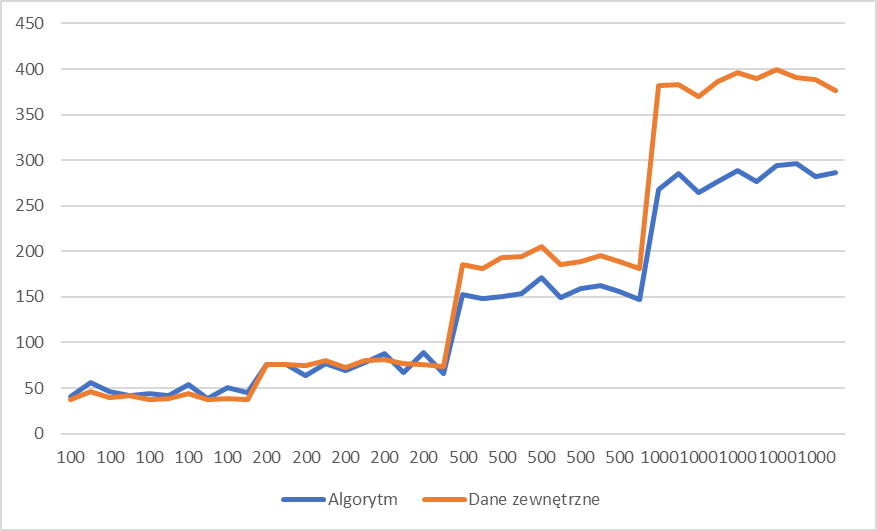
\includegraphics[scale=0.3]{1-100_20.png}
    \caption{Dane dla 1 - 100 z 20 maszynami}
    \label{1-100_20}
\end{figure}


\begin{figure}[h]
    \centering
    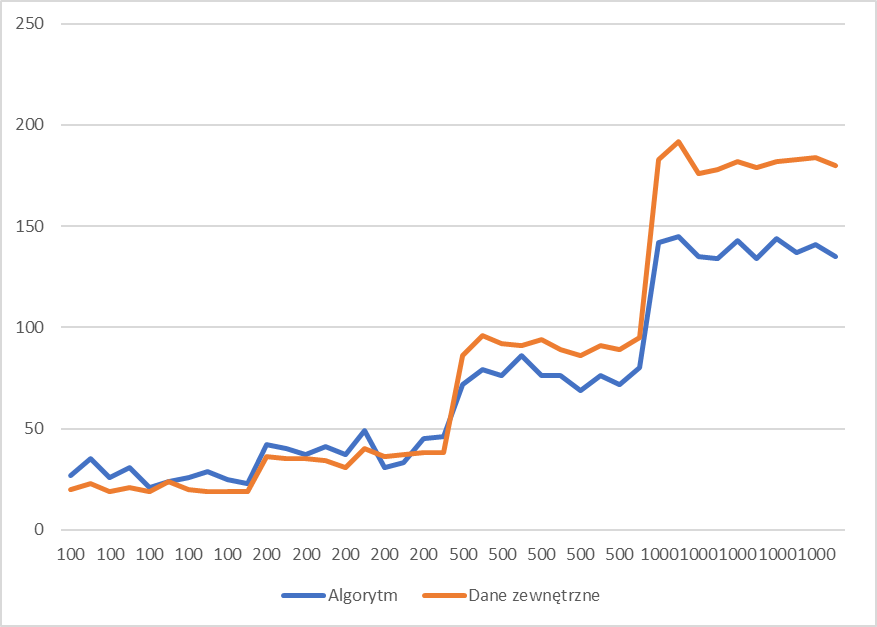
\includegraphics[scale=0.3]{1-100_30.png}
    \caption{Dane dla 1 - 100 z 30 maszynami}
    \label{1-100_30}
\end{figure}

\begin{figure}[h]
    \centering
    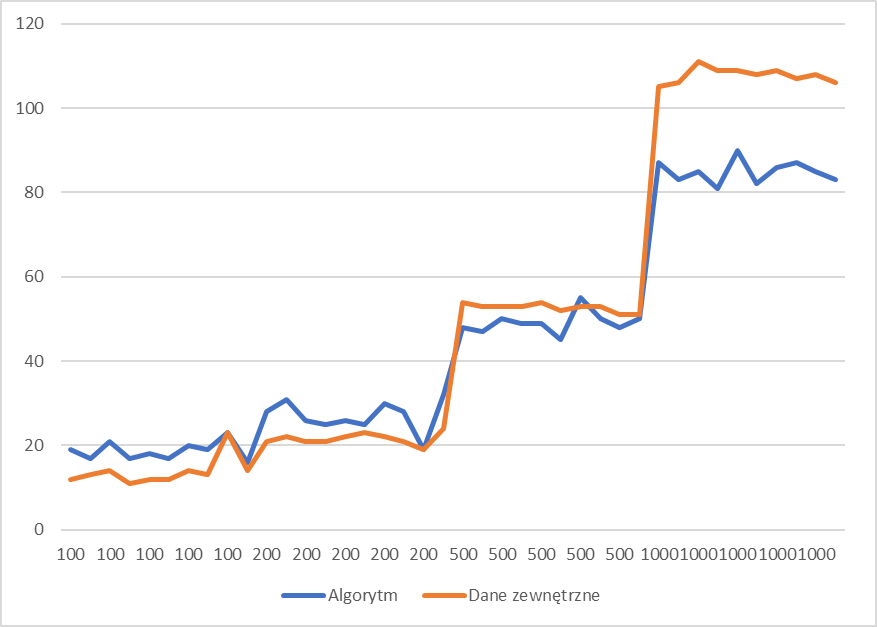
\includegraphics[scale=0.3]{1-100_40.png}
    \caption{Dane dla 1 - 100 z 40 maszynami}
    \label{1-100_40}
\end{figure}



\begin{figure}[h]
    \centering
    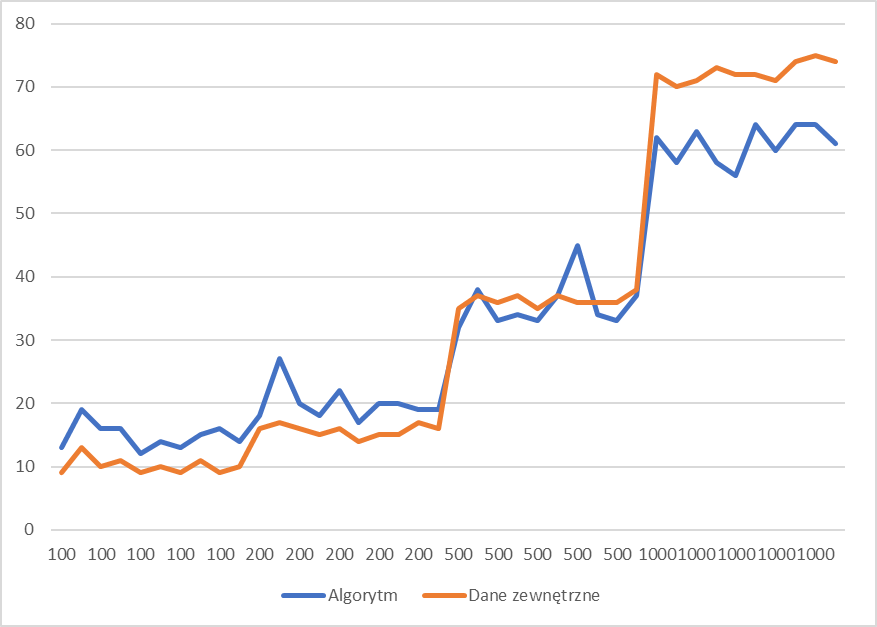
\includegraphics[scale=0.3]{1-100_50.png}
    \caption{Dane dla 1 - 100 z 50 maszynami}
    \label{1-100_50}
\end{figure}



\begin{figure}[h]
    \centering
    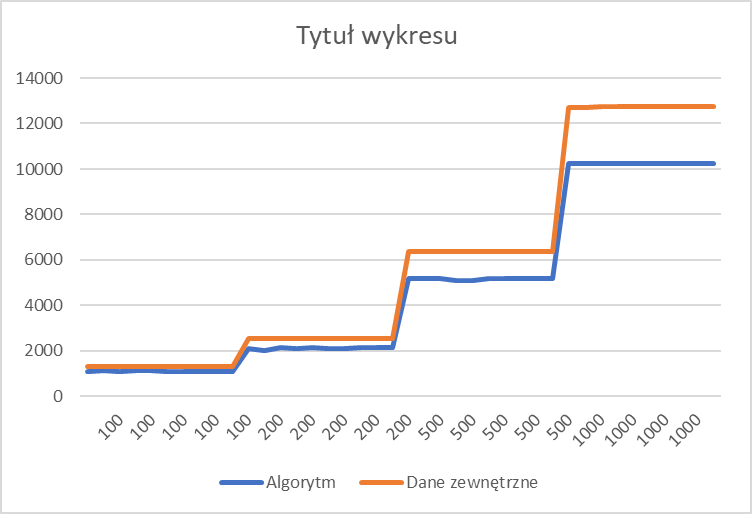
\includegraphics[scale=0.3]{100-120_10.png}
    \caption{Dane dla 100 - 120 z 10 maszynami}
    \label{100-120_10}
\end{figure}

\begin{figure}[h]
    \centering
    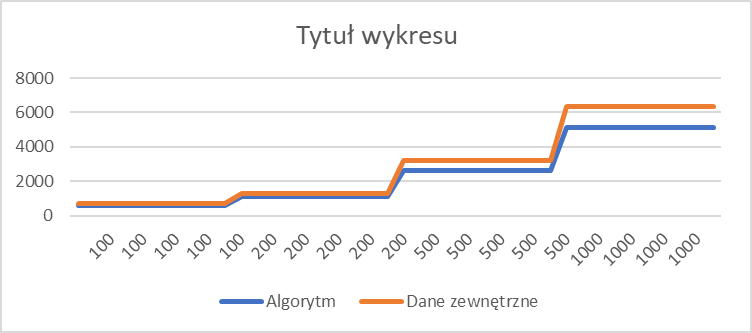
\includegraphics[scale=0.3]{100-120_20.png}
    \caption{Dane dla 100 - 120 z 20 maszynami}
    \label{100-120_20}
\end{figure}

\begin{figure}[h]
    \centering
    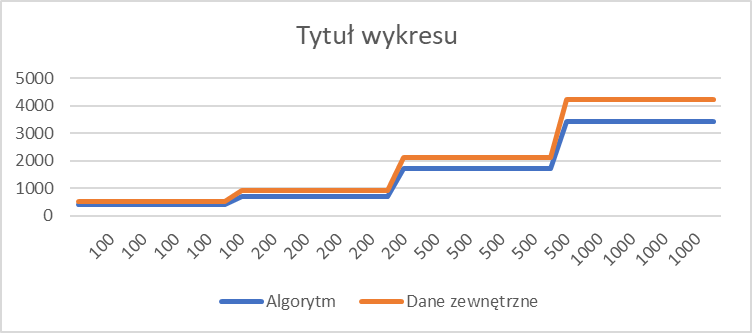
\includegraphics[scale=0.3]{100-120_30.png}
    \caption{Dane dla 100 - 120 z 30 maszynami}
    \label{100-120_30}
\end{figure}

\begin{figure}[h]
    \centering
    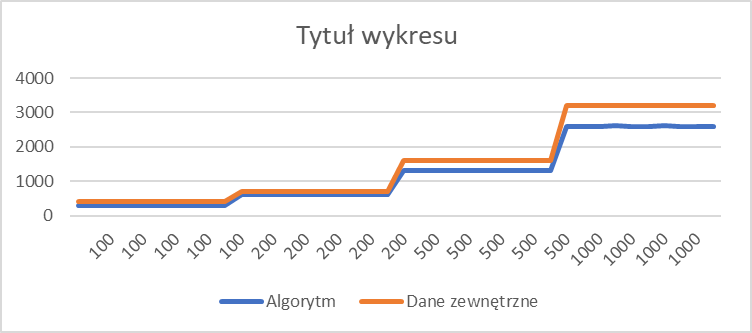
\includegraphics[scale=0.3]{100-120_40.png}
    \caption{Dane dla 100 - 120 z 40 maszynami}
    \label{100-120_40}
\end{figure}

\begin{figure}[h]
    \centering
    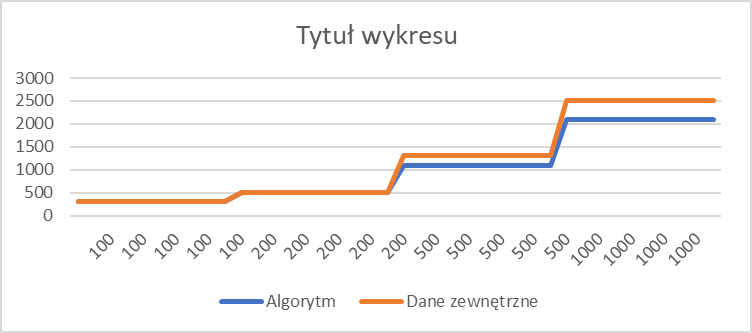
\includegraphics[scale=0.3]{100-120_50.png}
    \caption{Dane dla 100 - 120 z 50 maszynami}
    \label{100-120_50}
\end{figure}


\begin{figure}[h]
    \centering
    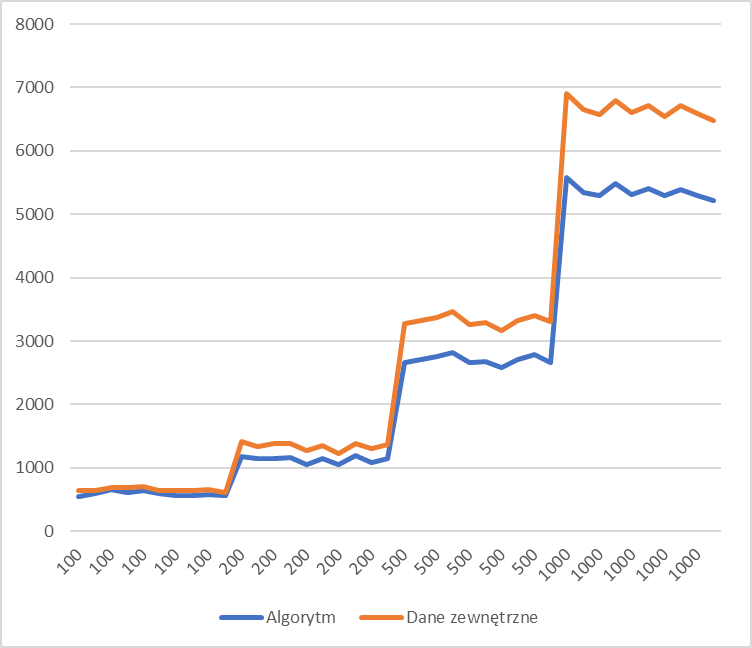
\includegraphics[scale=0.3]{jobs_10.png}
    \caption{Dane dla JobsCorre z 10 maszynami}
    \label{jobs_10}
\end{figure}

\begin{figure}[h]
    \centering
    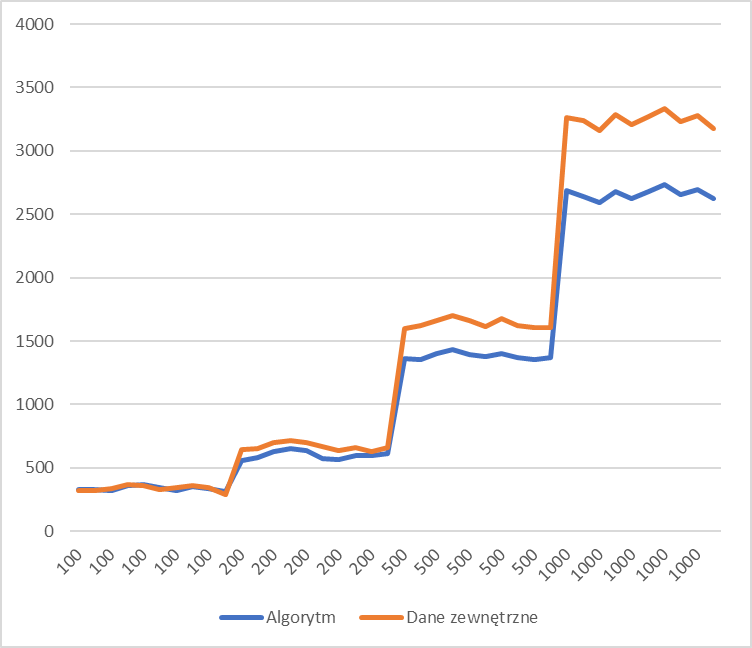
\includegraphics[scale=0.3]{jobs_20.png}
    \caption{Dane dla JobsCorre z 20 maszynami}
    \label{jobs_20}
\end{figure}

\begin{figure}[h]
    \centering
    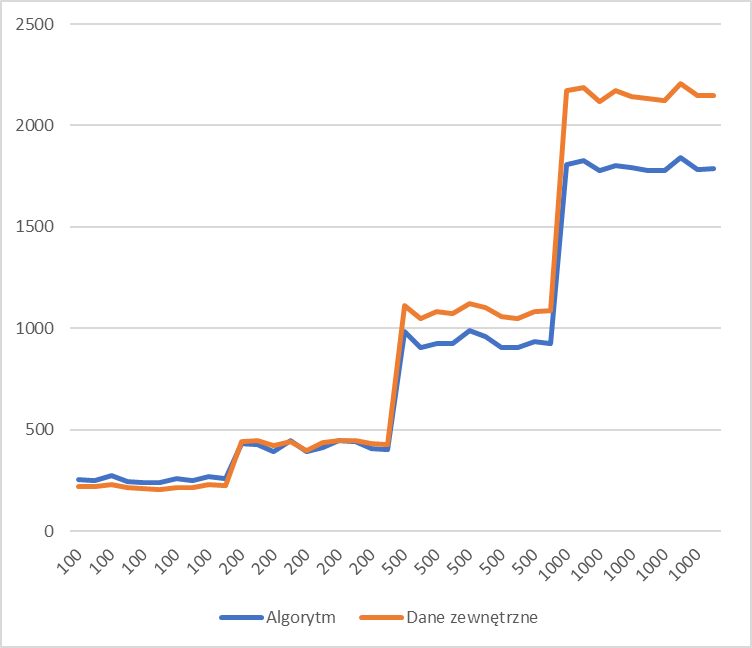
\includegraphics[scale=0.3]{jobs_30.png}
    \caption{Dane dla JobsCorre z 30 maszynami}
    \label{jobs_30}
\end{figure}

\begin{figure}[h]
    \centering
    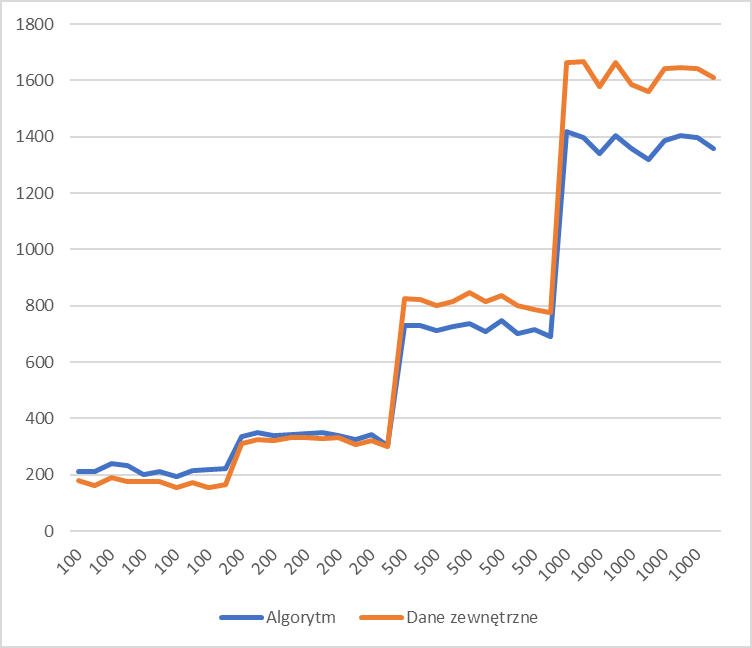
\includegraphics[scale=0.3]{jobs_40.png}
    \caption{Dane dla JobsCorre z 40 maszynami}
    \label{jobs_40}
\end{figure}

\begin{figure}[h]
    \centering
    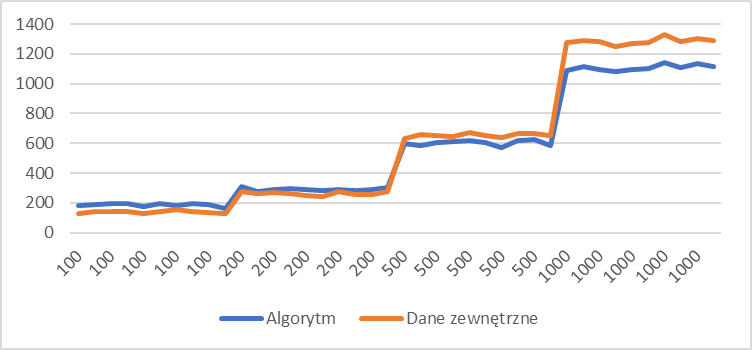
\includegraphics[scale=0.3]{jobs_50.png}
    \caption{Dane dla JobsCorre z 50 maszynami}
    \label{jobs_50}
\end{figure}


\begin{figure}[h]
    \centering
    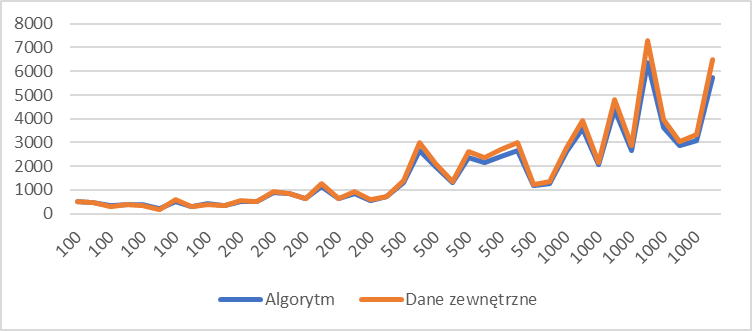
\includegraphics[scale=0.3]{moq_10.png}
    \caption{Dane dla MaqCorre z 10 maszynami}
    \label{moq_10}
\end{figure}

\begin{figure}[h]
    \centering
    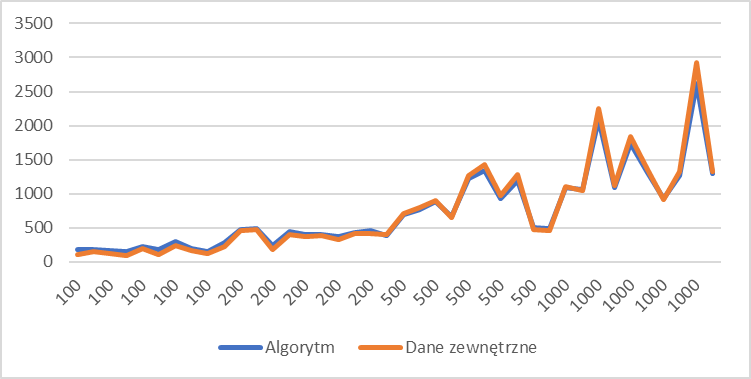
\includegraphics[scale=0.3]{moq_20.png}
    \caption{Dane dla MaqCorre z 20 maszynami}
    \label{moq_20}
\end{figure}

\begin{figure}[h]
    \centering
    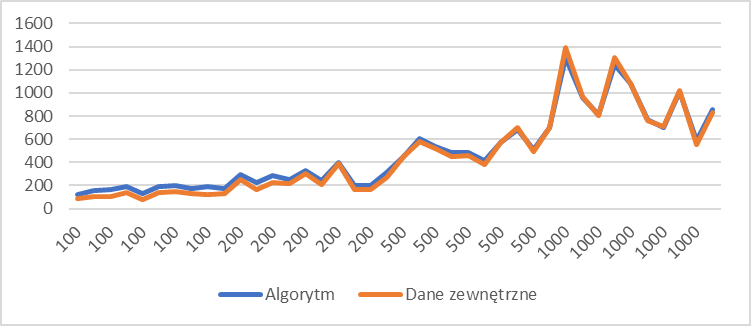
\includegraphics[scale=0.3]{moq_30.png}
    \caption{Dane dla MaqCorre z 30 maszynami}
    \label{moq_30}
\end{figure}

\begin{figure}[h]
    \centering
    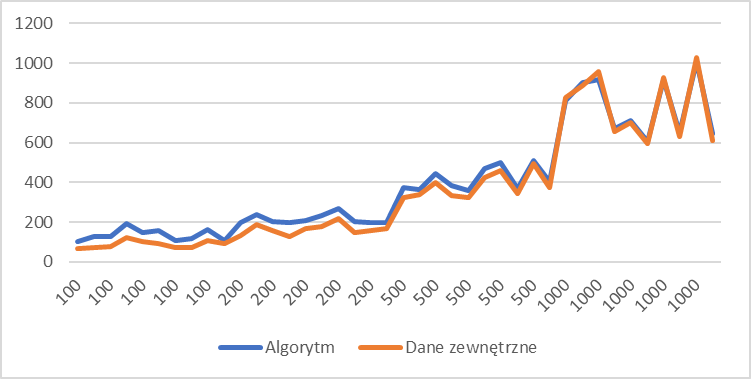
\includegraphics[scale=0.3]{moq_40.png}
    \caption{Dane dla MaqCorre z 40 maszynami}
    \label{moq_40}
\end{figure}

\begin{figure}[h]
    \centering
    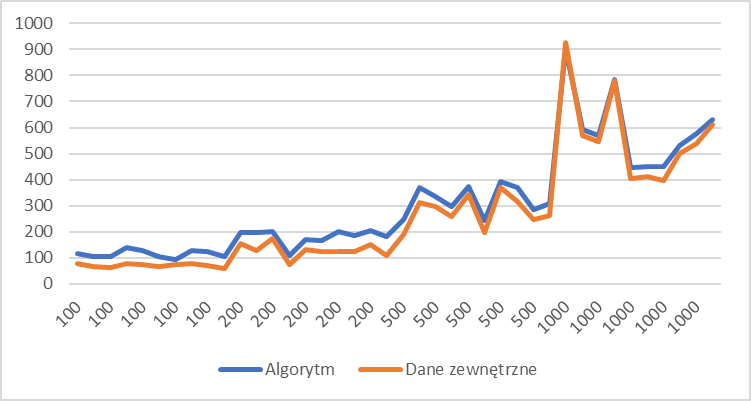
\includegraphics[scale=0.3]{moq_50.png}
    \caption{Dane dla MaqCorre z 50 maszynami}
    \label{moq_50}
\end{figure}
